%LaTeX template : http://systbio.org/files/SB_LaTeX_Template_txt_extension.txt
%Author instructions: http://www.oxfordjournals.org/our_journals/sysbio/for_authors/ms_preparation.html

\documentclass[12pt,letterpaper]{article}
\usepackage{natbib}

%Packages
\usepackage{pdflscape}
\usepackage{fixltx2e}
\usepackage{textcomp}
\usepackage{fullpage}
\usepackage{float}
\usepackage{latexsym}
\usepackage{url}
\usepackage{epsfig}
\usepackage{graphicx}
\usepackage{amssymb}
\usepackage{amsmath}
\usepackage{bm}
\usepackage{array}
\usepackage[version=3]{mhchem}
\usepackage{ifthen}
\usepackage{caption}
\usepackage{hyperref}
\usepackage{amsthm}
\usepackage{amstext}
\usepackage{enumerate}
\usepackage[osf]{mathpazo}
\usepackage{dcolumn}
\usepackage{lineno}
\pagenumbering{arabic}


%Pagination style and stuff
\linespread{2}
\raggedright
\setlength{\parindent}{0.5in}
\setcounter{secnumdepth}{0} 
\renewcommand{\section}[1]{%
\bigskip
\begin{center}
\begin{Large}
\normalfont\scshape #1
\medskip
\end{Large}
\end{center}}
\renewcommand{\subsection}[1]{%
\bigskip
\begin{center}
\begin{large}
\normalfont\itshape #1
\end{large}
\end{center}}
\renewcommand{\subsubsection}[1]{%
\vspace{2ex}
\noindent
\textit{#1.}---}
\renewcommand{\tableofcontents}{}
%\bibpunct{(}{)}{;}{a}{}{,}

%---------------------------------------------
%
%       START
%
%---------------------------------------------

%Submitting to: Evolution (thorough method + applied data)
%               Proc B (nice story + thorough method in the supplementaries?)
%               MEE (new method (time slicing) + increment on former methods (disparity)) 

% NC: Make sure to format for whichever journal we choose...

\begin{document}

%Running head
\begin{flushright}
Version dated: \today
\end{flushright}
\bigskip
\noindent RH: Tempo and mode in mammalian evolution

\bigskip
\medskip
\begin{center}

\noindent{\Large \bf Cretaceous-Palaeogene extinction does not affect mammalian disparity.} 
% NC: still think this might need some work

\bigskip

\noindent {\normalsize \sc Thomas Guillerme$^1$$^,$$^2$$^*$, and Natalie Cooper$^1$$^,$$^2$}\\
\noindent {\small \it 
$^1$School of Natural Sciences, Trinity College Dublin, Dublin 2, Ireland.\\
$^2$Trinity Centre for Biodiversity Research, Trinity College Dublin, Dublin 2, Ireland.}\\
\end{center}
\medskip
\noindent{*\bf Corresponding author.} \textit{Zoology Building, Trinity College Dublin, Dublin 2, Ireland; E-mail: guillert@tcd.ie; Fax: +353 1 6778094; Tel: +353 1 896 2571.}\\
\vspace{1in}

%Line numbering
\modulolinenumbers[1]
\linenumbers

%---------------------------------------------
%
%       ABSTRACT
%
%---------------------------------------------

\newpage
\begin{abstract}
% NC: As ever I'm ignoring this until we are finished with the rest!
%Massive global extinctions have a turn-over effect on biodiversity. When some large group of taxa suffers from a high rate of extinction, it is expected that niches becomes available for potentially unrelated clades that can undergo an adaptive radiation to fill these vacant niches.
%Therefore, in a context of current global biotic and abiotic changes, resolving this question is crucial to understand the effect of mass extinction events on biodiversity.
%The causes and effects of such events are well understood for marine organisms with a good fossil record (e.g. Ammonoidea and Foraminifera) but the effects remains unclear on some iconic vertebrate groups.

%Typically, placental mammals (eutherians) are shown by some studies to be undergoing an adaptive radiation after the Cretaceous-Palaeogene mass extinction event (K-Pg) by originating shortly before the K-Pg event and displaying high morphological evolutionary rates leading to high diversification during the Palaeogene. However, some other studies have demonstrated that eutherians originates during the Cretaceous and don't display significantly high diversification after the K-Pg event.

%Here we propose a new approach to test if eutherians undergo an adaptive radiation after the K-Pg event. We use trees containing both living and fossil taxa based on all the available data (Total Evidence) and the state-of-the-art method in dating (tip dating) along side with a better proxy for niche occupancy (morphological diversity as opposed to taxonomic diversity) and finer grain analysis through time (introducing a time slicing method).

%Our results shows that eutherians don't display significantly higher changes in morphological disparity that expected under a Brownian motion after the K-Pg boundary. We therefore propose that eutherian mammals don't undergo an adaptive radiation during the Palaeogene.

%Why is our stuff better?
%1-More accurate timing (TEM+tip dating vs. molecular node date or morphological parsimony)
%2-Better proxy for niche occupancy (morphological disparity + diversity vs. species diversity) (but niches concept is shite anyway)
%3-Better measure for disparity (centroid distance vs. Foote's quartet)
%4-Two evolutionary models instead of one for looking at disparity through time (punctuated+constant vs. punctuate)
%5-Systematic time units for looking at disparity through time (slices vs. intervals)

\end{abstract}

\noindent (Keywords: disparity, diversity, punctuated equilibrium, gradualism, time slicing)\\
% NC: Note that keywords are things that aren't in the title of the paper
\vspace{1.5in}

\newpage 

%---------------------------------------------
%
%       INTRODUCTION
%
%---------------------------------------------

\section{Introduction}

%-Macroevolution / niches / crisis in biodiversity
%-Diversity in mammals is known to increase blablabla (Stadler)
%Cheeky selling line: in the context of the anthropocene extinction event, blabalbal
%-However, not much is known about the disparity. We think disparity is a more functional measure of biodiversity since it is expected that more disparate species occupies more disparate niches and therefore have a globally more important role in the ecosystems.
%-We use a novel approach for looking at disparity as the spread of the data in a N dimensional character-space (centroid - Finlay Cooper)
%-Problem with timing the events (O'Leary vs Meredith). Here we look at disparity on total evidence trees that contain morphological information but are backed-up by molecular data.

% TG: I reworked the whole thing. It seems a bit short to me but I guess that'll need some adjusting/precisions.
% NC: I think the length is fine. Short = good.

% 1§ mass extinctions = bad. Loss of species (e.g. P/T 95%). But what comes after is more interesting: sp richness can increase, decrease or stay constant. So can sp niche occupancy. But it is not always link (ruta and stuff). Opportuinities, interaction, ecological role etc... A classical example is the rise of mammals
%Mass extinctions result in catastrophic declines in global biodiversity \citep{RaupPT,BentonPT,rennetime2013,Brusatte2015}. % TG: Maybe find a more catchy sentence.
Throughout history, life on earth has suffered a series of sudden catastrophic extinction events resulting in drastic declines in global biodiversity \citep[e.g.][]{RaupPT,BentonPT,rennetime2013,Brusatte2015}. % TG Maybe that one is better? Sudden and catastrophic contransting with long-term and varied in the second sentence?
However, the long-term effects of mass extinctions are more varied \citep{Erwin1998344}, and include increases in species richness in some clades \citep{friedmanexplosive2010}, species richness declines in others \citep{Benton85}, changes in morphological diversity \citep{brusattedinosaur2012} and shifts in ecological dominance \citep[e.g.][]{Brusatte12092008,toljagictriassic-jurassic2013,bensonfaunal2014}.
These shifts are characterized by the decline of one clade that is replaced by a different unrelated clade with a similar ecological role \citep{Brusatte12092008} (e.g. Brachiopoda and Bivalvia at the end Permian extinction \citealt{Sepkiski1981,CLAPHAM01102006} but see \citealt{Payne22052014}). They are of particular interest because they are a fairly common pattern observed in the fossil record \citep[e.g.][]{D'Hondt01011996,Coxall01042006,thorneresetting2011,bensonfaunal2014} and are often linked to major macroevolutionary processes such as adaptive radiation \cite{Losos2010} or competitive radiation \cite{Brusatte12092008}.

% 2§ explaining the rise of the age of the mammals view.
One classical example of a shift in ecological dominance is at the Cretaceous-Palaeogene (K-Pg) mass extinction 66 million years ago (Mya) \citep{rennetime2013}, where the non-avian dinosaurs went extinct, potentially leading to the ``rise of the age of the mammals" \citep{archibald2011extinction,Lovergrove}. 
This is based on the idea that placental mammals were able to diversify after the extinction of many terrestrial vertebrates at the K-Pg boundary (including the dominant non-avian dinosaur group \citep{archibald2011extinction,O'Leary08022013,Brusatte2015}. 
Some authors suggest this reflects placental mammals filling the ``empty'' niches left after the K-Pg event \citep{archibald2011extinction}, others suggest it reflects a release from predation and/or competition \citep{Lovergrove}.
However, evidence for the diversification of placental mammals after K-Pg is mixed.
Thorough analysis of the fossil record \citep[e.g.][]{goswamia2011,O'Leary08022013} supports the idea that placental mammals diversified after K-Pg as there are no undebated placental mammal fossils before the K-Pg event and many afterwards \citep{archibald2011extinction,goswamia2011,Slater2012MEE,O'Leary08022013,Wilson2013,Brusatte2015}. 
Conversely, evidence from molecular data suggests that the diversification of placental mammals started prior to the K-Pg extinction event without being drastically affected by it \citep{Douady2003285,bininda2007delayed,meredithimpacts2011,Stadler12042011,beckancient2014}. 
Therefore, whether the diversification of placental mammals began before K-Pg, or in response to the extinctions at K-Pg, is a matter of great debate \citep{O'Leary08022013,Springer09082013,O’Leary09082013}. 

There are three main reasons why there is still debate about the timing of the diversification of placental mammals. In this paper we focus on solving these issues as follows: % NC: Needs a bit more finesse but you get the idea 
  \begin{enumerate}
    \item \textbf{Palaeontological and neontological data show different patterns.}
    As mentioned above, conclusions about when placental mammals diversified tend to be split depending on what kind of data are used: palaeontological data generally suggest that placental mammals diversified post K-Pg \citep[e.g.][]{O'Leary08022013}, whereas neontological data suggest that K-Pg event had no effect on mammalian diversification \citep{bininda2007delayed,meredithimpacts2011,Stadler12042011}. 
    Fortunately we can deal with this issue by using all the data available, rather than using just fossils or molecules. 
    Here we use Total Evidence phylogenies containing cladistic data for both living and fossil taxa along with molecular data for living taxa \citep{eernissetaxonomic1993,ronquista2012}, and state-of-the-art tip-dating \citep{ronquista2012,Wood01032013} to get accurate estimates of diversification times for both fossil and living species.
    \item \textbf{Diversity can be defined in different ways.}
    Diversity is a difficult concept to define; in many studies diversity is measured as taxonomic diversity or species richness \citep{Stadler12042011,meredithimpacts2011,O'Leary08022013}, but often the more interesting aspect of diversity is related to the ecological niche the species occupy \citep{Wesley-Hunt2005,Brusatte12092008,toljagictriassic-jurassic2013} in order to draw hypothesis about the macroevolutionary processes \citep{Pearman2008149,OlsonRadiation,Losos2010,glor2010phylogenetic}.
    In addition, it is important to note that species richness variations can be decoupled from variations in morphological diversity \citep{slaterCetacean,ruta2013,hopkinsdecoupling2013}, so using only species richness may not be the best proxy for ecological diversity.
    In this study we therefore measure the variations in morphological diversity, also refereed as disparity \citep{Wills1994,BIJ:BIJ455,Wesley-Hunt2005,brusatte50,cisneros2010,prentice2011,anderson2012using,Hughes20082013,bentonmodels2014} as a way to quantify the changes in diversity in an ecological sense.
    \item \textbf{Methods are outdated and make inappropriate assumptions}
    Finally, the methods used to quantify these changes where proposed more than 20 years ago \cite{Foote01071994,Wills1994} and are sometimes reused without revision \citep{brusatte50,Brusatte12092008,cisneros2010,thorneresetting2011,prentice2011,brusattedinosaur2012,toljagictriassic-jurassic2013,ruta2013,bentonmodels2014,bensonfaunal2014} even if they violate some basic statistic assumptions such as variables independence.
    Previous methods also make the assumption that changes in disparity are punctual rather than continuous \citep{Wagner01011997,Wesley-Hunt2005}.
    Finally most of these studies that focused on changes of disparity through time used unequal time units based on biostratigraphy \citep{Brusatte12092008,brusattedinosaur2012,toljagictriassic-jurassic2013}.
    One can argue that this can be tautological since biostratigraphy is already based on changes in fossil assemblages and morphology through time.
    In this study we revise the statistical methods for measuring disparity.
    Also, we propose a new method called ``time-slicing'' allowing to look at changes in disparity through time in a continuous way along with the possibility of specifying the evolutionary model (punctuated or constant).
  \end{enumerate}

Here, we propose an updated approach to test whether mammals diversified before or after K-Pg, using morphological disparity as our measure of diversity.
We measured the cladistic disparity of two previously published studies \citep{Slater2012MEE,beckancient2014} based on both molecular and morphological data and using the Total Evidence trees dated using the tip-dating method \citep{ronquista2012,Wood01032013}.
Using a novel ``time-slicing'' approach we provide a fine grain estimation disparity through time and also allows us to make different assumptions about the evolutionary models underlying morphological character evolution (either constant or punctuated). 
Finally, to test whether mammals display significant changes in disparity after the K-Pg boundary, we compared the observed changes to two null model assuming purely stochastic or purely Brownian evolution. 
We found no significant increase in cladistic disparity after the K-Pg event and in fact the disparity in eutherian mammals spiked during the K-Pg event. 
These results suggest that the shift in dominant terrestrial vertebrate clades in the vertebrate fossil record during the Tertiary (from non-avian dinosaurs to eutherian mammals) is not due to the K-Pg extinctions.

%---------------------------------------------
%
%       METHODS
%
%---------------------------------------------

\section{Methods}

%To put somewhere:
%Methodological improvements
%Distance matrix: we use Graeme's MORD that more accurately reflects distances between taxa - Actually just Gower from now since Graeme's paper's not out for a while
%Disparity: we use the centroid distance that is a clear and easily-interpretable method that is less dependent from diversity (see supplementaries)
%Time: we use Total Evidence Tip dated trees that are more accurate because they use probabilistic methods to estimate morphological phylogenetic distance (Wright) and provide more accurate ages of diversification events (Ronquist).
%Disparity through time: Finally, we use a *novel method* (to our knowledge) to look at the diversity through time. Instead of calculating the disparity of all species present in a time interval (e.g. Butler and Brusatte), we calculate disparity at a set of arbitrary and equidistant points in time. This new method provides a finer grain resolution of the evolution of diversity through time as well as two well defined models of character evolution (pucntuated - random, acctran, deltran - and continuous - proximity) contrary to the time interval method that assumes only punctuated as a evolutionary model for morphological characters and can be biased towards biostratigraphy.


% NC: I'm not sure that this is necessary for this paper. It's much more linear that the previous one. You could save for the supp mat or your thesis 
%To test whether mammals display a significant change in disparity after the K-Pg boundary we use the following protocol (note that each step is explained in detail below this section; Fig.~\ref{fig_method}.
%\begin{enumerate}
%\item{Data: we used the cladistic morphological matrices and the Total Evidence tip-dated trees published in \citep{Slater2012MEE} and \citep{beckancient2014}.} \\
%\item{Estimating ancestral character states: we used the \citep{Yang01121995} re-rooting method to estimate the states of each characters in the cladistic morphological matrices at each node and created the reconstructed morphological matrix containing observed morphological characters data for tips in the tree and estimated morphological characters states for nodes.}\\
%\item{Calculating the cladisto-space: using the reconstructed morphological matrix we defined the cladisto-space by using a principal components ordination of the Gower distance matrix \citep{Gower71} representing the $n$ finite dimensional space that encompasses the total cladistic morphological variation of the taxa present in the analysis.} \\
%\item{Time slicing: we then separated the cladisto-space into subdivisions containing only the edges (nodes or/and tips) present every 5 million years from present (hereafter called "time-slices").} \\
%\item{Disparity through time: we then calculate the phylogenetic diversity as the number of edges present at each time-slice as well as the cladistic morphological disparity defined as the spread of the edges in the cladisto-space at each time-slice (distance from cladisto-space centroid \citep{finlay2015morphological}.} \\
%\item{Null model testing: finally, we compared the observed disparity to the expected disparity under two different null models: (1) the first one being a completely stochastic model where disparity is random at each point in time.; and (2) the second one being a $Mk_n$ model (as a proxy for Brownian evolution) where disparity increase is constant through time.} \\
%\end{enumerate}

%\begin{figure}[!htbp]
%\centering
%    \includegraphics[keepaspectratio=true]{Figures/MEthod_outline.pdf}
%\caption{General method outline. The grey section represents the Total Evidence data and tip dated trees from two published studies \citep{Slater2012MEE,beckancient2014}. \textbf{A}: We then estimated the ancestral characters states from the observed morphological matrices from both studies. we then calculated the distance matrix using the Gower distance \citep{Gower71} and performed a ordination of the distance matrix to create the cladisto-space. Finally, we divided the cladisto-space matrix using the Time slicing method to measure the changes in morphological disparity through time. \textbf{B}: we then generated two sets of a hundred simulated "null" matrices under two null models, the random matrix: a fully stochastic matrix; and the $Mk_n$ matrix: a matrix simulated under the $Mk_n$ model. We then applied the same procedure as for \textit{A} (ordinated distance matrix and time slicing) to calculate the disparity through time expected for purely random data and for a constant evolution model. Finally we compared our simulated disparity through time to our observed disparity through time to estimate if mammals displayed a significant increase in disparity after the K-Pg boundary.}
%\label{fig_method}
%\end{figure}

\subsection{Cladistic data an phylogenies}
We used the cladistic morphological matrices and the Total Evidence tip dated trees \citep{ronquista2012} from \citep{Slater2012MEE} (103 taxa and 446 morphological characters) and \citep{beckancient2014} (102 taxa and 421 morphological characters).
We chose these two data sets because they have a similar number of taxa and morphological characters.
\cite{Slater2012MEE} ranges from 310 Million years ago (Mya - Late Carboniferous) to the present and focuses on Mammaliamorpha up to the family level.
\cite{beckancient2014} ranges from 170 Mya (Middle Jurassic) to the present and focuses on Eutheria up to a genus level.
We used the first and last occurrences as the temporal span of each taxon in our analysis \citep{Slater2012MEE,beckancient2014}.


\subsection{Estimating ancestral character states}
For both datasets we estimated the ancestral state of each character at every node in the tree using Maximum Likelihood.
We used the \texttt{rerootingMethod} function from the R package \texttt{phytools} version 0.4-45 \citep{phytools}.
This method performs a Maximum Likelihood estimation of the ancestral values and the variance of a Brownian motion process based on the re-rooting method of \citep{Yang01121995}.
% NC: May need a bit more info here. Also you need to cite garland's original paper here too. TG: Not sure which Garland's paper??
We followed the method of \citep{Claddis} for treating missing data at the tips as any possible observed state for each character.
For example if a character has a maximum of two observed states (0 and 1), we attributed the multi-state ``0\&1" value to the tips with missing data giving an equal probability of being either 0 or 1.
This allows the ancestral descendant to a tip with missing data to be still estimated.
We preferred Maximum Likelihood methods to Bayesian methods because both methods have been shown to produce similar results \citep{royer-carenzichoosing2013} but Maximum Likelihood methods are several orders of magnitude faster than Bayesian ones (total analysis time $~$1.2 CPU year). 

In order to remain conservative with the ancestral states reconstruction (especially when a high error is associated to the ancestral state), we only considered the ancestral state reconstruction with a scaled likelihood $\geq$ than 0.95.
We replaced the ancestral states reconstruction below this threshold by ``NA".
However, for a matter of comparison, we also provided the results of the analysis without removing the ancestral state reconstruction with low scaled likelihoods intervals ($\leq$ 0.95). % link to supp

\subsection{Estimating the cladisto-space}
To explore the variation in mammalian disparity (defined here as the variation in morphology) through time, we use a cladisto-space approach \citep{Foote01071994,Foote29111996,Wesley-Hunt2005,Brusatte12092008,Hughes20082013,friedmanexplosive2010,toljagictriassic-jurassic2013}.
This approach is similar to a morphospace based on continuous morphological data \citep[e.g.][]{friedmanexplosive2010,finlay2015morphological}, except the cladisto-space is based on cladistic data (i.e. the discrete morphological characters used to build a phylogenetic tree).
Mathematically, the cladisto-space is a $n$ dimension object that summarizes the distances between the taxa present in the cladistic matrix (see details below).
Because of it's inherent combinatory properties, a cladisto-space is a finite theoretical object limited by the product of the number of character states. In fact, a cladisto-space will be overloaded if the number of taxa is higher than the product of the number of character states. Therefore it is straightforward to make sure that the character space does not contain more taxa than it's maximal capacity.
Estimating the cladisto-space requires two steps described in detail below: (1) calculating the distance matrix and (2) applying multidimensional scaling.

\subsubsection{Distance matrix}
We first calculate the pairwise distance matrix among all taxa using the Gower distance \citep{Gower71}. The Gower distance is the Euclidean distance between two taxa divided by the number of comparable not identical characters. 
In the case of cladistic matrices, this corrected distance is preferable because of it's ability to deal with discrete or/and ordinated characters as well as with missing data \citep{anderson2012using}
The Gower distance is correcting the distance between two taxa that share many characters and that will therefore being (just by chance) more close to other taxa with which they don't share many characters.
%We also calculated the Generalised Euclidean Distance (GED) \citep{Wills2001} and the MORD distance (@Lloyd in prep.@) to make our results comparable with previous studies (e.g.) % TG: or maybe not.
Cladisto-space methods can suffer from problems due to inapplicable characters, for example, some pairwise distances between taxa can not be calculated if the pairs of taxa don't have any available data in common.
To solve this problem we used the \texttt{TrimMorphDistMatrix} function from the \texttt{Claddis R} package \citep{Claddis}.
This function removes the taxa that contain the most non-calculable distance until the distance matrix contains no ``NAs".

\subsubsection{Multidimensional scaling}
We then transformed the distance matrices using classic multidimensional scaling \citep{torgerson1965multidimensional,GOWER01121966,cailliez1983analytical}.
The multidimensional scaling (also refereed as MDS, PCA or PCO) is an orthogonal transformation of the variance co-variance matrix calculated from the distance matrix.
Because covariance between certain taxa can be negative, we corrected the distance matrix using the Cailliez correction \cite{cailliez1983analytical} which multiply all the covariance values by a constant. %as in \citep{toljagictriassic-jurassic2013}
This allows to calculate $n$ eigen vector (i.e. the $n$ dimensions of the cladisto-space) where $n$ is equal to a maximum of the size of the distance matrix (which is in our case the number of taxa in each matrix) \textit{minus} the two last eigen vectors (that are null after applying the Cailliez correction).

These two steps allowed us to calculate the cladisto-space for both datasets. 
ote that the $n$ dimensional objects represent the total variation of the morphological diversity (disparity) for all the mammals present in the data.
In other words, our cladisto-space represent an ordination of all the possible mammalian morphologies coded in each studies, not the cladistic disparity at any point in time.
In order to measure the cladistic disparity through time, we measured the observed subsection of the cladisto-space at each point in time.
These observed cladistic disparity can never be greater than the total disparity in the cladisto-space.
We explain the calculation of the disparity as well as it's measure through time below.

\subsection{Disparity}
We measured the cladistic morphological disparity (i.e. the diversity in discrete morphological characters) by using the distance from centroid \citep{finlay2015morphological}.
The distance from centroid is defined as the mean euclidean distance between each edge (nodes and tips) and the centroid which is the mean value of each dimension of the cladisto-space:
\begin{equation}
Disparity=\frac{\sum{\sqrt{(Edge_{n}-Centroid_{n}^2}}}{Number\ of\ edges}
\end{equation}
Where $Edge_{n}$ is any edge value in the $n^{th}$ dimension of the cladisto-space and $Centroid_{n}$ is the average value of the $n^{th}$ dimension. Note that the disparity is calculated using all the $n$ dimensions of the cladisto-space (i.e. we used all axis of the ordination).

We used this metric for measuring disparity rather than the classically used sum and product of ranges and variance \cite{Foote01071994,Wills1994,brusatte50,Brusatte12092008,cisneros2010,thorneresetting2011,prentice2011,brusattedinosaur2012,toljagictriassic-jurassic2013,ruta2013,bentonmodels2014,bensonfaunal2014} because


because this method is less correlated with diversity (see supplementary) and allows to use the data of all the dimensions of the cladisto-space without being incalculable for the dimensions that bear a little amount of the distance variance. For example, the product of range and variance are always equal to zero if the last dimensions of the character space bare a minimal amount of the variance of the distance matrix (traditionally less than 5\%). Also this method is clearer and easier to interpret \citep{finlay2015morphological}. For comparing our results to previous studies, we also calculated the sum and product of ranges and variance, these results are available in the supplementary materials.

For each disparity measurement, we bootstrapped 1000 times the subdivision of the cladisto-space containing only the edges present at each time slice. We then calculated the 50\% and 95\% confidence interval associated with each disparity measurement.

\subsubsection{Diversity}
We counted phylogenetic diversity as the number of phylogenetic elements in each subdivision of the cladisto-space (i.e. branches, nodes and tips per slice). We logged our diversity measurements to make the differences additive instead of multiplicatives.
%Because both datasets used did not contain all living mammals, we also calculated the number of phylogenetic element per million year from the Fritz supertree \citep{fritzdiversity2013} (see details on the calculations in the supplementary materials). %TG: Useless, see above.


\subsection{Time slicing} % NC: I feel like maybe this should be combined with disparity? So explain the general principle, then go back to explain in detail? TG: Not sure, what the time slicing is actually doing is to separate the ordinated distance matrix into submatrices that contains only taxa present at the slice. The disparity can be calculated either on the slices or on the overall results.
We propose a new approach to look at changes in disparity
% NC: Somewhere you need to clearly define disparity
through time by calculating the spread of the cladisto-space at time points in the phylogeny rather than considering the spread of the cladisto-space in time intervals or bins \citep[e.g.][]{Brusatte12092008,brusattedinosaur2012,toljagictriassic-jurassic2013}. The time intervals approach suffers from several biases: (1) time interval duration is set arbitrarily and can distort the diversity or disparity in that time interval. For example, if stratigraphical ages are used, it is likely to increase the differences between two strata since they are traditionally based on differences in the morphology of fossils found in the different strata; (2) the time intervals method assumes that all characters evolve following a punctuated equilibrium model, i.e. if a character 
% NC: If a character does what???
between two time intervals, the character state is assumed to be constant for the whole duration of the interval and then evolve quickly to reach the state in the subsequent time interval; \citep{Gould1977}. % NC: Why is this a problem?
% NC: Maybe better to reorder this as "Previous studies have done X. This is bad because this and this and this". Instead we propose a new method.

To address these issues, we propose a time slicing method that only considers subdivisions of the cladisto-space at specific equidistant points in time (as opposed to the time intervals that considers  subdivisions of the cladisto-space between two points in time; see Fig.~\ref{fig_slicing}. This methods addresses two of the biases introduced by the time intervals method: (1) it allows to sample evenly through time elements in the phylogeny without arbitrarily grouping certain edges together. For example, the slice at 0 Mya will contain only the extant taxa instead of an interval defined as the Quaternary (from 2.5 Mya to the present) that will also include extinct taxa. However, it is highly probable for vertebrate data that no data is available at any point in time. Therefore we propose two models of character evolution to estimate the state of a character at any point in time along a branch, addressing at the same time the second potential bias in the time intervals method: (2) at any specific point in time, a branch is sampled instead of an edge, we propose two different models to determine whether to consider the data from the ancestor edge or the descendant one.
\begin{enumerate}
\item{Punctuated model:} this model selects either the data from the ancestor or the descendant edge. Similarly to the time interval method, this model reflects punctuated evolution where the changes occur either at the start or at the end of a branch. In practice, we randomly chose the data from the ancestor or the descendant edge each time. However, we also tested the model with the assumption that changes always occurs early on the branch (accelerate transition, ACCTRAN) or are always delayed towards the descendant edge (delayed transition, DELTRAN). The result of both assumption are available in the supplementary material.
\item{Constant model:} this models selects either the data from the ancestor or the descendant edge according to the branch length separating the sampling point and the ancestor's edge. If the sampling point along the branch is lower than half the branch length, then the data from the ancestor edge is selected. Else we selected the data from the descendant edge. This model reflects constant evolution where changes rate are constant and cumulative along the branch (i.e. the hypothetical character state at any point in time will likely to be the same to the closest observed state in time - ancestor or descendant edge).
\end{enumerate}

\begin{figure}[!htbp]
\centering
    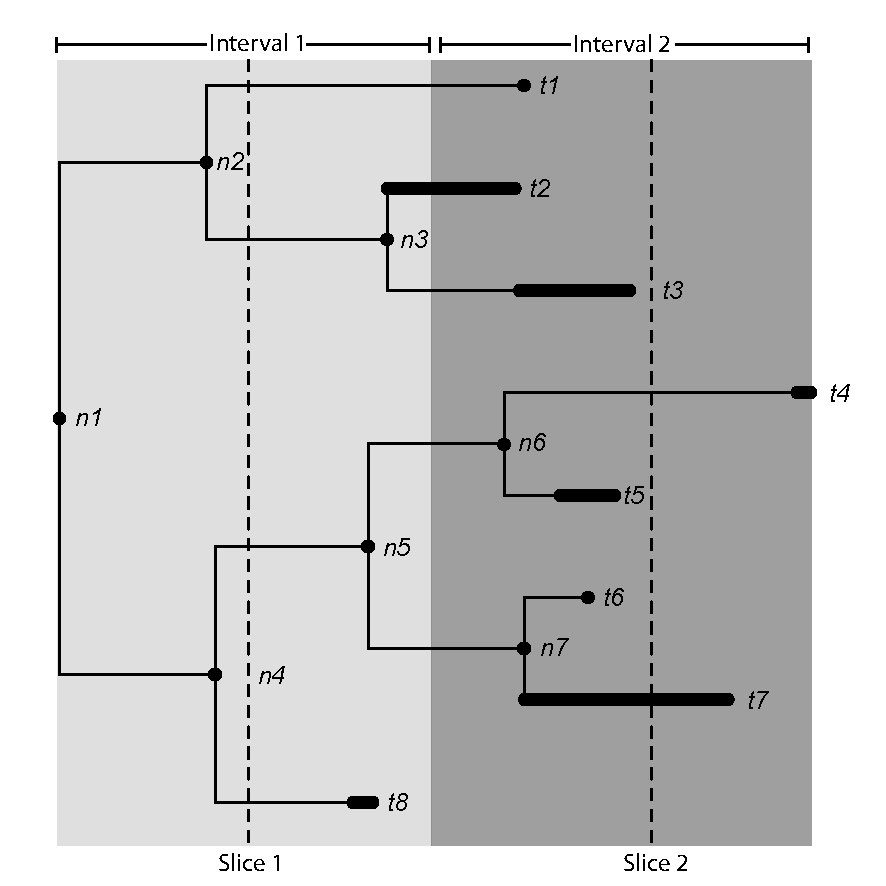
\includegraphics[keepaspectratio=true]{Figures/Slicing.pdf}
\caption{Differences in slicing method and intervals. Solid lines represent the First and Last Appearance Datum span. Interval 1 contains the following elements within the global character-space: taxa t2 and t8 and nodes n1, n2, n3, n4 and n5. Interval 2 contains the following elements within the global character-space: taxa t1, t2, t3, t4, t5, t6 and t7 and nodes n6 and n7. Slice 1 contains the following elements within the global character-space under the proximity model (constant evolution assumption): nodes n2 and n4. Slice 2 contains the following elements within the global character-space under the proximity model (constant evolution assumption): taxa t4 and t7.}
\label{fig_slicing}
\end{figure}

We applied this time slicing method to both cladisto-spaces \citep{Slater2012MEE,beckancient2014} using a time interval of 5 Mya (from present to 170 Mya) slicing each cladisto-space in 35 subdivisions. We also performed a time intervals approach to compare our results to previous publications \citep[e.g.][]{Brusatte12092008,brusattedinosaur2012,toljagictriassic-jurassic2013}. The results of this analysis are available in the supplementary materials.

\subsubsection{Rarefaction}
To avoid bias due to the number of edges variation in each cladisto-space subdivision we also re-sampled each subdivision to have an equal number of phylogenetic elements available (edges or branches). Each subdivision was therefore re-sampled to contain the minimal number of taxa in the smallest subdivision. Because this led in certain cases to a absolute minimum of phylogenetic elements to calculate disparity (3) we also arbitrarily re-sampled the subdivisions to contain 10 elements or less. In practice, for both cases, we bootstrapped the disparity measurements by randomly removing $x$ elements per subdivision, where $x$ is either (1) the number of edges sampled in each time slice minus the minimum of edges in each time slice or (2) the number of edges to remove so that the number of elements is not higher than 10. Both results are available in the supplementary materials.

\subsection{Null models testing}
Finally, we tested the effect of the K-Pg boundary on mammal disparity, by measuring whether the observed changes were significantly different than expected by chance. We rerun the full disparity analysis (minus the ancestral states reconstruction part) on both phylogenies with the same number of edges and the same time slices. However, we replaced the observed character matrices by two times 100 randomly generated ones following two null models. The first null model (repeated 100 times) was a purely stochastic matrix where each cell value was sampled from a discrete uniform distribution with a number of sates equal to the number of states observed in the the original data. For the second null model, we simulated each characters for each edge using the phylogenetic structure using the \texttt{sim.character} function from the \texttt{diversitree R} package \citep{fitzjohndiversitree2012} and the $Mk_n$ \citep{lewisa2001} with an equal transition rate between the number of characters states observed in the original matrix and a unique rate ($\mu$) sampled from a uniform distribution (0 $<$ $\mu$ $\leq$ 0.5). 
We then measured the amount of overlap between both null models and the observed data using the Bhattacharyya Coefficient \citep{Bhattacharyya} which measures the probability of overlap between two distributions (similarly as a two sided \textit{t-test}; \citep{GuillermeCooper}. We considered the observed data to be non different than random for a Bhattacharyya Coefficient $>$0.95 and on the opposite, we considered a significant difference in disparity than expect by chance when the Bhattacharyya Coefficient was $<$0.05.

% OR actually maybe just go for anova...
%---------------------------------------------
%
%       RESULTS
%
%---------------------------------------------

\section{Results}

%---------------------------------------------
%
%       DISCUSSION
%
%---------------------------------------------

\section{Discussion}

%Disparity improvements
%Previous studies have calculated disparity on a subset of PCO axes \citep[e.g.][]{Brusatte12092008} but in this study we calculated it on all the available axis (i.e. the full n dimensional cladisto-space) to avoid excluding outliers.

%Biases:
%-internal versus terminal branches
%-ancestral states reconstruction (solved by being conservative?)
%-poor sampling of living taxa (Guillerme & Cooper)

%From Wilson 2013
%My results reveal several key findings: (1) latest Cretaceous mammals, particularly metatherians and multituberculates, had a greater ecomorphological diversity than is generally appreciated, occupying regions of the morphospace that are interpreted as strict carnivory, plant-dominated omnivory, and herbivory; (2) the decline in dental-shape disparity and body-size disparity across the K/Pg boundary shows a pattern of constructive extinction selectivity against larger-bodied dietary specialists, particularly strict carnivores and taxa with plant-based diets, that suggests the kill mechanism was related to depressed primary productivity rather than a globally instantaneous event; (3) the ecomorphological recovery in the earliest Paleocene was fueled by immigrants, namely three multituberculate families (taeniolabidids, microcosmodontids, eucosmodontids) and to a lesser extent archaic ungulates; and (4) despite immediate increases in the taxonomic richness of eutherians, their much-celebrated post-K/Pg ecomorphological expansion had a slower start than is generally perceived and most likely only began 400,000 to 1 million years after the extinction event.


%Therefore, the cladisto-space is likely to be more influenced by phylogeny than the morphospace \citep{Foote29111996,Wagner01011997}. However, discrete cladistic characters are still the best source for quantifying overall morphology for large and diverse groups \citep{Brusatte12092008}. % NC: Make this justification better. why does the phylogney effect matter. Should this be mentioned here at all? TG: not specially, might be something a reviewer might point out. I remember you pointing it out ;). However, STD is become fairly common these days so maybe people have accepted the idea.

%---------------------------------------------
%
%       CONCLUSION
%
%---------------------------------------------

\section{Conclusion}


%---------------------------------------------

\section{Data availability and reproducibility}

\section{Acknowledgments}
Graeme Lloyd, Gavin Thomas, Sive Finlay.
%Simulations used the Lonsdale cluster maintained by the Trinity Centre for High Performance Computing and funded through grants from Science Foundation Ireland. %TG: I think they won't in the end

\section{Funding} % NC: Usually this is part of acknowledgments.
This work was funded by a European Commission CORDIS Seventh Framework Programme (FP7) Marie Curie CIG grant (proposal number: 321696).

 %   \citept{key} ==>>                Jones et al. (1990)
 %   \citept*{key} ==>>               Jones, Baker, and Smith (1990)
 %   \citep{key} ==>>                (Jones et al., 1990)
 %   \citepp*{key} ==>>               (Jones, Baker, and Smith, 1990)
 %   \citepp[chap. 2]{key} ==>>       (Jones et al., 1990, chap. 2)
 %   \citep[e.g.][]{key} ==>>        (e.g. Jones et al., 1990)
 %   \citepp[e.g.][p. 32]{key} ==>>   (e.g. Jones et al., p. 32)
 %   \citepauthor{key} ==>>           Jones et al.
 %   \citepauthor*{key} ==>>          Jones, Baker, and Smith
 %   \citepyear{key} ==>>             1990

\bibliographystyle{sysbio}
\bibliography{References}

\section{supplementaries}

\subsection{Ancestral states estimation}
We used both the \texttt{ace} function from the R package ape v. 3.2 \citep{paradisape:2004} and the 
\texttt{rerootingMethod} function from the R package phytools 0.4-45 \citep{phytools}. Both method perform a maximum likelihood estimation of the ancestral values and the variance of a Brownian motion process based on the re-rooting method of \citep{Yang01121995}. The two methods differ slightly in the calculation of the normalized conditional likelihoods but mainly on the way to treat missing data. We optimised the \texttt{ace} function for fast estimation by treating missing data in the matrix as an extra character (e.g. if a character has two observed tips states 0 and 1 and a third tip has missing data (NA), the ancestor of these three tips can be estimated between the three following states: 0, 1 and NA). For the \texttt{rerootingMethod}, we followed \citep{Claddis} method and treated the missing in the tips as any possible observed state (e.g. if a character has two observed tips states 0 and 1 and a third tip has missing data (NA), the third tip will be considered as multi-state (0\&1) and the ancestor of these three tips can be estimated between the two following states: 0 and 1). Both methods perform similarly but the implementation of the \texttt{ace} function has a slightly lower accuracy  but is three times faster than the one for the \texttt{rerootingMethod} function (see supplementaries).
% NC: Some of this probably belongs in methods

\subsubsection{Time intervals}
We then divide our observed cladisto-spaces into sub cladisto-spaces representing the different stages of the character-space filling. For example, if at various points in time.
%The intervals should be a compromise between the resolution and the sample size and must be "sufficiently coards that nearly all generic first and last occurenaces can be unambiguously assigned" \citep{Foote01071994}.
Time intervals from 170Ma (Earliest Cenomanian, Late Cretaceous) to the present.
We count all the nodes/tips present in a given time interval.
Classic but artificially grouping data. The minimal bin size should contain at least two nodes/tips and sometime that involves having time intervals spanning accross tens of millions of years. Such long duration time intervals have no real biological meaning since it is unlikely that all of the nodes/tips present in the time interval did ever coexisted and had ever biological interactions together.

\subsection{Diversity}
-Diversity in living mammals
-Diversity per interval

\subsection{Disparity}
-Centroid is less correlated with diversity
-Other metrics

\subsection{Not to be in the paper, neither in the supplementaries (methods table)}

\begin{table}[ht]
\caption{Comparison of Cladisto-space studies methods}
\centering
\begin{tabular}{cccccccc}
  \hline
    Date & Author      & Distance  & Ordination & Binning    & Disparity   & Difference & cite \\ %
  \hline
         & this study  & Gower     & PCO        & Time slice & centroid    & NPMANOVA?  & \\
    2014 & Benson      &           &            & Equal bins & Wills 1994* & NPMANOVA   & \citep{bensonfaunal2014} \\
    2014 & Brusatte    & Euclidean & PCO        &            &             &            & \citep{brusattegradual2014} \\
    2014 & Benton      & Euclidean & PCO        & Biostrat   & Wills 1994* & NPMANOVA   & \citep{bentonmodels2014} \\
    2013 & Hopkins     &           &            & Equal bins & Wills 1994* &            & \citep{hopkinsdecoupling2013} \\             
    2013 & Ruta        & GED       & PCO        & Biostrat   & Wills 1994* & NPMANOVA   & \citep{ruta2013} \\
    2013 & Hughes      & Euclidean & PCO        & Biostrat   & Sum of var  &            & \citep{Hughes20082013} \\
    2013 & Toljagic    & Euclidean & PCO        & Biostrat   & Wills 1994* & NPMANOVA   & \citep{toljagictriassic-jurassic2013} \\
    2012 & Brusatte    & Euclidean & PCO        & Biostrat   & Wills 1994* & CI overlap & \citep{brusattedinosaur2012} \\
    2012 & Anderson    & Gower     & PCO        &            &             &            & \citep{anderson2012using} \\
    2010 & Prentice    & Euclidean & PCO        & Biostrat   & Wills 1994* & NPMANOVA   & \citep{prentice2011} \\
    2011 & Thorne      & Euclidean & PCO        & Biostrat   &             & NPMANOVA   & \citep{thorneresetting2011} \\
    2010 & Cisneros    & Euclidean & PCO        & Biostrat   & Wills 1994* & NPMANOVA   & \citep{cisneros2010} \\
    2008 & Brusatte    & Euclidean & PCO        & Biostrat   & Wills 1994* & NPMANOVA   & \citep{brusatte50} \\
    2008 & Brusatte    & Euclidean & PCO        & Biostrat   & Wills 1994* & NPMANOVA   & \citep{Brusatte12092008} \\
    2005 & Wesley-Hunt &           & PCO        &            & Foote 1992  & t-test     & \citep{Wesley-Hunt2005} \\
  \hline
\end{tabular}
\end{table}
* The 4 sum and product of range and variance




\end{document}
